\documentclass[12pt, letterpaper]{article}
\usepackage{inputenc, amsmath, amssymb, bm, mathrsfs, mathtools, hyperref, amsthm}
\usepackage[margin=.8 in]{geometry}
\usepackage{enumerate}
\usepackage{graphicx}
\usepackage[font=footnotesize,labelfont=bf]{caption}
\usepackage{subcaption}
\usepackage{titlesec}
\usepackage{setspace}
\usepackage{tikz}
\setlength\parindent{0pt}

\newtheorem{theorem}{Theorem}[section]
\newtheorem{corollary}{Corollary}[theorem]
\newtheorem{lemma}[theorem]{Lemma}
\newtheorem{definition}{Definition}[section]
\newtheorem{example}{Example}[section]

% Will def need this later, should probably do this rn though :(
% \usepackage[backend=biber]{biblatex}
% \let\cite=\supercite
% \addbibresource{refs.bib}

\newcommand\myeq{\stackrel{\mathclap{\normalfont\mbox{def}}}{=}}
\newcommand{\R}{\mathbb{R}}
\newcommand{\C}{\mathbb{C}}
\newcommand{\Half}{\mathbb{H}}
\newcommand{\Z}{\mathbb{Z}}
\newcommand{\Q}{\mathbb{Q}}
\newcommand{\N}{\mathbb{N}}
\newcommand{\ten}[1]{\textnormal{\textbf{#1}}}


\title{Notes}
\author{Preston Malen}
\date{January 2024}

\begin{document}

\maketitle
\thispagestyle{empty}

\newpage
\thispagestyle{empty}
\section*{Introduction}
First and foremost I want to clarify that by no means am I an expert on the presented
topics or any topics in mathematics for that matter. I have wanted to study complex
geometry for quite some time but was unable take a course or do research in the area.
So this is me exploring complex geometry and some of the topics that are parallel.
Most of this information is new to me at the time of writing. Also worth noting,
I am writing this with a VERY casual approach so my language and verbiage may not be
as formal or precise, I'm writing what my brain is thinking. I am documenting my
journey of learning complex geometry and whatever may branch off of it. I'm starting
with a quick refresher on some important ideas from differential geometry such as
charts, atlases etc. From there, a quick review of some complex analysis then an
interlude with some exterior algebra. Exterior algebra is something I have had
little to so it will be interesting to explore it's connection to geometry.
Nothing too technical is needed from exterior algebra to study complex geometry at a beginner
level, however we do need exterior powers and exterior products at the minmum. Then
from there I will start to dive into complex manifolds and Kähler geometry. It was
to my suprise that complex geometry relied heavily on topics from algebraic geometry,
so that will be quite the learning curve as well. From Kähler geometry, I am going
to go wherever my interest takes me. If I find something interesting along the way,
I will more than likely dive into it a little deeper.

\newpage
\thispagestyle{empty}
\tableofcontents


\newpage
\clearpage




\newpage

\section{Foundations of Differential Geometry}


\section{Complex Analysis Review}
Before we can go too deep in Kähler manifolds (and some Riemannian geometry in
general), we need to have a quick review of complex analysis.

\subsection{Holomorphic Functions}

\begin{definition}\label{def 3.1}
    Given an open set $\Omega \in \C$, a function $f: \Omega \to \C$ is \ten{analytic}
    if for all $z_0 \in \Omega$ there exists a ball of radius $\varepsilon>0$ about
    $z_0$ such that $f$ has a well-defined power series:
    \begin{equation*}
        f(z) = \sum_{n=0}^\infty a_n (z-z_0)^n, \quad \forall z \in B_\varepsilon
        (z_0)
    \end{equation*}
\end{definition}

Some refer to this definition as a \textbf{holomorphic} function but this is technically
incorrect. Analyticity is a local property defined about some $\varepsilon$-neighbordhood
whereas being holomorphic is a little more general. The differentiable property of
complex functions is defined only pointwise. A classical example of this difference
would be a function that is only differentiable about a line and thus not analytic. 
However, in complex analysis these two definitions (analytic and holomorphic) happen
to be equivalent so they are often use interchangeabley. The proof is not too difficult
but we omit it here. We will however establish the exact definition of holomorphic.

\begin{definition}\label{3.2}
    A function $f: \Omega \to \C$, typically expressed as $f(x,y) = u(x,y) + iv(x,y)$,
    is \ten{holomorphic} if it satisfies the Cauchy-Riemannan
    equations:
    \begin{equation*}
        \dfrac{\partial u}{\partial x} = \dfrac{\partial v}{\partial y}, \quad
        \dfrac{\partial u}{\partial y} = - \dfrac{\partial u}{\partial x}
    \end{equation*}
\end{definition}
In fact, we can generalize this to $\C^n$. Now let $f: \Omega \subseteq \C^n \to
\C^n$. This function is holomorphic on $\C^n$ if it satisfies the generalized 
Cauchy-Riemann equations:
\begin{equation*}
    \dfrac{\partial u}{\partial x_i} = \dfrac{\partial v}{\partial y_i}, \quad 
    \dfrac{\partial u}{\partial y_i} = - \dfrac{\partial v}{\partial x_i},\quad
    \text{for } i = 1, 2, \hdots , n
\end{equation*} 
In laymen's terms, $f$ is holomorphic in every ``direction'' or coordinate. This
gives us a perfect segue into how the complex Jacobian matrix for a holomorphic function
$f$ is related to and defined by the Cauchy-Riemann equations:
\begin{equation*}
    J(f)(z):= \bigg(\dfrac{\partial f_i}{\partial z_j}(z)\bigg), \ 1 \leq i \leq n, \
    1 \leq j \leq m
\end{equation*}
Recall from differential geometry that Jacobian matrices define transition maps.
The complex Jacobian matrices also play a part in complex manifolds as we will see
later.

\section{Exterior Algebra Interlude}

\section{Complex Manifolds}
Now we have all the tools to study complex manifolds via their charts, transition
maps, and morphisms. First we will look at the complex equivalents of some foundational
definitions in differential geometry. We start by defining an analogue for an atlas.

\begin{definition}
    A \ten{holomorphic atlas} on a differentiable manifold $M$ is an atlas
    $\{(\Omega_i, \varphi_i)\}$ such that $\Omega_i \cong \varphi_i(\Omega_i) \subseteq
    \C^n$ and the transition functions are holomorphic.
\end{definition}

\vspace{.5cm}

\tikzset{every picture/.style={line width=0.75pt}} %set default line width to 0.75pt        

\begin{center}
\begin{tikzpicture}[x=0.75pt,y=0.75pt,yscale=-1,xscale=1]
%uncomment if require: \path (0,300); %set diagram left start at 0, and has height of 300

%Shape: Polygon Curved [id:ds20814686542469296] 
\draw   (140,68) .. controls (160,58) and (250,48) .. (230,68) .. controls (210,88) and (216,97.6) .. (236,127.6) .. controls (256,157.6) and (143,170.6) .. (123,140.6) .. controls (103,110.6) and (120,78) .. (140,68) -- cycle ;
%Shape: Polygon Curved [id:ds16655262050332986] 
\draw   (402,65) .. controls (411,34.4) and (426,78.6) .. (478,58.6) .. controls (530,38.6) and (521,114.6) .. (541,144.6) .. controls (561,174.6) and (365,156.2) .. (385,124.6) .. controls (405,93) and (393,95.6) .. (402,65) -- cycle ;
%Curve Lines [id:da8606798953332562] 
\draw    (232,94) .. controls (271.6,64.3) and (324.92,59.69) .. (380.32,89.68) ;
\draw [shift={(382,90.6)}, rotate = 208.97] [color={rgb, 255:red, 0; green, 0; blue, 0 }  ][line width=0.75]    (10.93,-3.29) .. controls (6.95,-1.4) and (3.31,-0.3) .. (0,0) .. controls (3.31,0.3) and (6.95,1.4) .. (10.93,3.29)   ;
%Shape: Polygon Curved [id:ds6793981765658346] 
\draw  [dash pattern={on 4.5pt off 4.5pt}] (188,113.6) .. controls (214,130.6) and (202,134.6) .. (175,138.6) .. controls (148,142.6) and (162,96.6) .. (188,113.6) -- cycle ;
%Shape: Polygon Curved [id:ds8163663421596739] 
\draw  [dash pattern={on 4.5pt off 4.5pt}] (459,128) .. controls (439,98) and (507,111.6) .. (499,132.6) .. controls (491,153.6) and (479,158) .. (459,128) -- cycle ;
%Curve Lines [id:da7463153933358471] 
\draw    (177,129) .. controls (138.19,190.29) and (213.24,146.05) .. (189.37,218.5) ;
\draw [shift={(189,219.6)}, rotate = 288.67] [color={rgb, 255:red, 0; green, 0; blue, 0 }  ][line width=0.75]    (10.93,-3.29) .. controls (6.95,-1.4) and (3.31,-0.3) .. (0,0) .. controls (3.31,0.3) and (6.95,1.4) .. (10.93,3.29)   ;
%Curve Lines [id:da8802878285570561] 
\draw    (480,131) .. controls (478.02,187.03) and (456.44,174.85) .. (445.33,217.3) ;
\draw [shift={(445,218.6)}, rotate = 284.04] [color={rgb, 255:red, 0; green, 0; blue, 0 }  ][line width=0.75]    (10.93,-3.29) .. controls (6.95,-1.4) and (3.31,-0.3) .. (0,0) .. controls (3.31,0.3) and (6.95,1.4) .. (10.93,3.29)   ;

% Text Node
\draw (298,43.4) node [anchor=north west][inner sep=0.75pt]    {$f$};
% Text Node
\draw (164,33.4) node [anchor=north west][inner sep=0.75pt]    {$X$};
% Text Node
\draw (449,34.4) node [anchor=north west][inner sep=0.75pt]    {$Y$};
% Text Node
\draw (193,96.4) node [anchor=north west][inner sep=0.75pt]    {$U$};
% Text Node
\draw (496,91.4) node [anchor=north west][inner sep=0.75pt]    {$V$};
% Text Node
\draw (178,230.4) node [anchor=north west][inner sep=0.75pt]    {$\mathbb{C}^{n}$};
% Text Node
\draw (437,230.4) node [anchor=north west][inner sep=0.75pt]    {$\mathbb{C}^{n}$};
% Text Node
\draw (303,216.4) node [anchor=north west][inner sep=0.75pt]    {$T_{J}$};
% Text Node
\draw (163,182.4) node [anchor=north west][inner sep=0.75pt]    {$\varphi $};
% Text Node
\draw (428,177.4) node [anchor=north west][inner sep=0.75pt]    {$\phi $};
% Connection
\draw    (203,239) -- (432,239) ;
\draw [shift={(434,239)}, rotate = 180] [color={rgb, 255:red, 0; green, 0; blue, 0 }  ][line width=0.75]    (10.93,-3.29) .. controls (6.95,-1.4) and (3.31,-0.3) .. (0,0) .. controls (3.31,0.3) and (6.95,1.4) .. (10.93,3.29)   ;

\end{tikzpicture}
\end{center}

\vspace{.5cm}

A map $f: X \to Y$ between differentiable manifolds, is holomorphic if the map:
\begin{equation*}
    \phi \cdot f \cdot \varphi^{-1}: \varphi(f^{-1}(U)\cap U)) \to \phi(V)
\end{equation*}
is holomorphic. Here the map $T_J$ is the transition map given by the Jacobian matrix.
Note that $\varphi$ and $\phi$ map to a respective open subset of $\C^n$ (perhaps all of $\C^n$).
\begin{definition}
Two differentiable manifolds $X$ and $Y$ are \ten{biholomorphic}
(or isomorphic) if there exists a holomorphic homeomorphism between them.
\end{definition}

So in the picture above, if $f$ is a holomorphic homeomorphism, that would imply
$X$ and $Y$ are biholomorphic.\\

Another really important topic in the study of manifolds is the idea of a submanifold.
In a very loose sense, we can think of these as subsets of manifolds.

\begin{definition}
    Let $X$ be a complex manifold with dimension $n$ and $Y \subseteq X$ a differentiable
    manifold of dimension $2k$. $Y$ is a \ten{complex submanifold} of $X$ of dimension
    $k$ if there exists a holomorphic atlas $\{ ( U_i, \varphi_i )\}$ of $X$ such
    that $\varphi: U_i \cap Y \cong \varphi(U_i) \cap \C^k$ is a biholomorphism.
\end{definition}

We identify $\C^k \subseteq \C^n$ as $(z_1, \hdots, z_k, 0, \hdots, 0)$ with zeroes
to the $n$-th coordinate.\\

Now we will shift gears just a little and look at some very foundational objects in 
complex geometry and algebraic geometry in general. These are some pretty heavy duty
ideas and they are not easy to grasp by any means. We will try to give visual representations
as much as possible, but note that it may take a lot of time to understand some of
the following theory and that's totally normal.\\

\begin{definition}
    Let $X$ be a topological space. A \ten{presheaf} $F$ of sets on $X$ conatins
    the following:
    \begin{itemize}
        \item For each open set $U$ of $X$, there exists a set $F(U)$ denoted
        $\Gamma(U,F)$. Elements of this set are \ten{sections} of $F$ over $U$.
        The sections of $F$ over $X$ are called the \ten{global sections} of $F$.
        \item For each inclusion of open sets $V \subseteq U$, there is a function
        $\textnormal{res}_{V,U} \hspace{-2pt}: \hspace{-2pt}F(U) \to F(V)$. These are \ten{restriction morphisms}.
        If $s \in F(U)$, this its restriction $\textnormal{res}_{V,U}$ is denoted $s \mid_V$.
    \end{itemize}
    The restriction morphisms must satisfy two additional properties:
    \begin{itemize}
        \item For every open $U \subseteq X$, the restriction morphism
        $\textnormal{res}_{U,U} \hspace{-5pt}:\hspace{-5pt} F(U) \to F(U)$ is the identity morphism on $F(U)$.
        \item For three open sets $W \subseteq V \subseteq U$, then we have
        $\textnormal{res}_{W,V} \circ \textnormal{res}_{V,U} = \textnormal{res}_{W,U}$.
    \end{itemize}
\end{definition}

Now for a concrete example, consider a set $U$, we can then assign the set $C^0(U)$
of all continuous real-valued functions on $U$. The restriction maps here are given
by restricting a continuous function on $U$ to a an open subset $V \subseteq U$.
In this case, $C^0(U)$ is a presheaf on the set $U$.\\

\begin{center}
    \tikzset{every picture/.style={line width=0.75pt}} %set default line width to 0.75pt        

    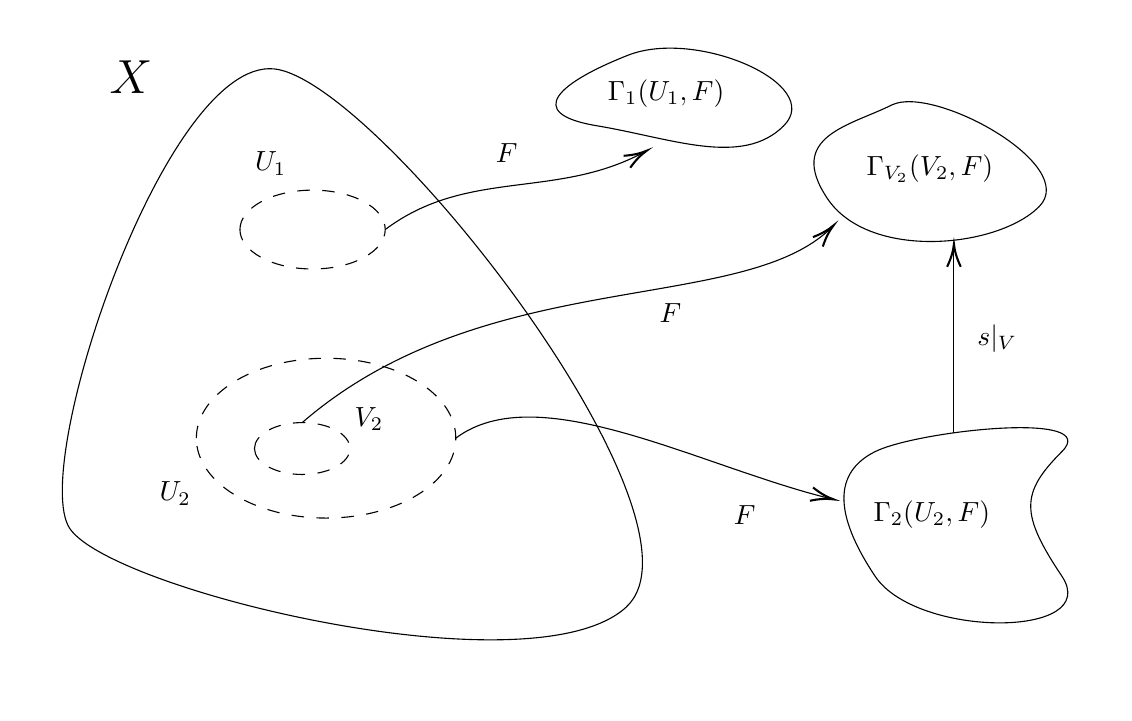
\begin{tikzpicture}[x=0.75pt,y=0.75pt,yscale=-1,xscale=1]
    %uncomment if require: \path (0,300); %set diagram left start at 0, and has height of 300
    
    %Shape: Polygon Curved [id:ds22855316313587815] 
    \draw   (269,18) .. controls (322,30) and (481,236) .. (436,277) .. controls (391,318) and (188,269) .. (168,239) .. controls (148,209) and (216,6) .. (269,18) -- cycle ;
    %Shape: Ellipse [id:dp8888433416673807] 
    \draw  [dash pattern={on 4.5pt off 4.5pt}] (250,95) .. controls (250,84.51) and (265.67,76) .. (285,76) .. controls (304.33,76) and (320,84.51) .. (320,95) .. controls (320,105.49) and (304.33,114) .. (285,114) .. controls (265.67,114) and (250,105.49) .. (250,95) -- cycle ;
    %Shape: Ellipse [id:dp44038825701634976] 
    \draw  [dash pattern={on 4.5pt off 4.5pt}] (257,200.5) .. controls (257,193.6) and (267.3,188) .. (280,188) .. controls (292.7,188) and (303,193.6) .. (303,200.5) .. controls (303,207.4) and (292.7,213) .. (280,213) .. controls (267.3,213) and (257,207.4) .. (257,200.5) -- cycle ;
    %Shape: Ellipse [id:dp22179985676130953] 
    \draw  [dash pattern={on 4.5pt off 4.5pt}] (229,195.5) .. controls (229,174.24) and (256.98,157) .. (291.5,157) .. controls (326.02,157) and (354,174.24) .. (354,195.5) .. controls (354,216.76) and (326.02,234) .. (291.5,234) .. controls (256.98,234) and (229,216.76) .. (229,195.5) -- cycle ;
    %Shape: Polygon Curved [id:ds9184016769940264] 
    \draw   (437,11) .. controls (470,-2) and (532,25) .. (512,45) .. controls (492,65) and (458,51) .. (422,45) .. controls (386,39) and (404,24) .. (437,11) -- cycle ;
    %Curve Lines [id:da9167721372681283] 
    \draw    (320,95) .. controls (359.6,65.3) and (402.14,80.68) .. (444.71,57.71) ;
    \draw [shift={(446,57)}, rotate = 150.83] [color={rgb, 255:red, 0; green, 0; blue, 0 }  ][line width=0.75]    (10.93,-3.29) .. controls (6.95,-1.4) and (3.31,-0.3) .. (0,0) .. controls (3.31,0.3) and (6.95,1.4) .. (10.93,3.29)   ;
    %Curve Lines [id:da543335583937063] 
    \draw    (280,188) .. controls (368.11,111.77) and (491.5,136.49) .. (534.72,94.3) ;
    \draw [shift={(536,93)}, rotate = 133.67] [color={rgb, 255:red, 0; green, 0; blue, 0 }  ][line width=0.75]    (10.93,-3.29) .. controls (6.95,-1.4) and (3.31,-0.3) .. (0,0) .. controls (3.31,0.3) and (6.95,1.4) .. (10.93,3.29)   ;
    %Shape: Polygon Curved [id:ds5031808706086047] 
    \draw   (564,35) .. controls (584,25) and (655,64) .. (635,84) .. controls (615,104) and (553,110) .. (533,80) .. controls (513,50) and (544,45) .. (564,35) -- cycle ;
    %Shape: Polygon Curved [id:ds06387135579224568] 
    \draw   (556,202) .. controls (576,192) and (666,182) .. (646,202) .. controls (626,222) and (626,232) .. (646,262) .. controls (666,292) and (576,292) .. (556,262) .. controls (536,232) and (536,212) .. (556,202) -- cycle ;
    %Curve Lines [id:da6009117343989652] 
    \draw    (354,195.5) .. controls (393.6,165.8) and (471.42,209.12) .. (534.11,224.54) ;
    \draw [shift={(536,225)}, rotate = 193.39] [color={rgb, 255:red, 0; green, 0; blue, 0 }  ][line width=0.75]    (10.93,-3.29) .. controls (6.95,-1.4) and (3.31,-0.3) .. (0,0) .. controls (3.31,0.3) and (6.95,1.4) .. (10.93,3.29)   ;
    %Straight Lines [id:da21625347797570593] 
    \draw    (594,193) -- (594,104) ;
    \draw [shift={(594,102)}, rotate = 90] [color={rgb, 255:red, 0; green, 0; blue, 0 }  ][line width=0.75]    (10.93,-3.29) .. controls (6.95,-1.4) and (3.31,-0.3) .. (0,0) .. controls (3.31,0.3) and (6.95,1.4) .. (10.93,3.29)   ;
    
    % Text Node
    \draw (186,12.4) node [anchor=north west][inner sep=0.75pt]  [font=\LARGE]  {$X$};
    % Text Node
    \draw (256,56.4) node [anchor=north west][inner sep=0.75pt]    {$U_{1}$};
    % Text Node
    \draw (426,21.4) node [anchor=north west][inner sep=0.75pt]    {$\Gamma _{1}( U_{1} ,F)$};
    % Text Node
    \draw (210,215.4) node [anchor=north west][inner sep=0.75pt]    {$U_{2}$};
    % Text Node
    \draw (304,179.4) node [anchor=north west][inner sep=0.75pt]    {$V_{2}$};
    % Text Node
    \draw (544,56.4) node [anchor=north west][inner sep=0.75pt]    {$ \begin{array}{l}
    \Gamma _{V_{2}}( V_{2} ,F)\\
    \\
    \end{array}$};
    % Text Node
    \draw (451,129.4) node [anchor=north west][inner sep=0.75pt]    {$F$};
    % Text Node
    \draw (480,224.4) node [anchor=north west][inner sep=0.75pt]    {$ \begin{array}{l}
    F\\
    \end{array}$};
    % Text Node
    \draw (554,224.4) node [anchor=north west][inner sep=0.75pt]    {$\Gamma _{2}( U_{2} ,F)$};
    % Text Node
    \draw (604,139.4) node [anchor=north west][inner sep=0.75pt]    {$s|_{V}$};
    % Text Node
    \draw (372,52.4) node [anchor=north west][inner sep=0.75pt]    {$F$};
    
    \end{tikzpicture}
\end{center}

Pictured above we have a visual of a presheaf defined on open subsets of a topological
space $X$. Here, the sets $F(U_i)$ are a presheaf over $X$. We also see the restriction
morphism $s\mid_V: \Gamma_2(U_2,F) \to \Gamma_{V_2}(V_2,F)$. Elements of any given
$\Gamma$ are sections of $F$ on the given $U$.\\

Presheaves are a great tool but they lack a little bit of power. We really want 
to extend this idea to an entire space or set to retrieve global information.

\begin{definition}
    A presheaf is a \ten{sheaf} if it satisfies the following:
    \begin{itemize}
        \item (Locality) Let $U$ be an open set, $\{U_i\}$ is an open cover of $U$
        with $U_i \subseteq U$ for all $i$, and $s,t \in F(U)$ are sections. If
        $s\mid_{U_i} = t \mid_{U_i}$ for all $i$ then $s=t$.
        \item (Gluing) Let $U$ be an open set, $\{U_i\}$ is an open cover of $U$
        with $U_i \subseteq U$ for all $i$, and $\{s_i \in F(U_i)\}$ is a family
        of sections. If all pairs of sections agree on the overlap of their domains,
        $s_i\mid_{U_i\cap U_j} = s_j\mid_{U_i\cap U_j}$ for all indices $i,j$, then
        there exists a section $s\in F(U)$ such that $s_i\mid_{U_i} = s_i$ for all $i$.
    \end{itemize}
\end{definition}

In a nutshell, presheaves assign data to sets locally while sheaves let us extend
this globally. We will mostly be concerned with a sheaf of holomorphic functions
$\mathcal{H}(-)$. However, there will certainly be more applications. Yes that is
a lot to take in.

\begin{definition}
    Let $X$ be a complex manifold. An \ten{analytic subvariety} of $X$ is a closed
    subset $Y \subseteq X$ such that for each $x \in X$, there exists an open neighbordhood
    $U \in X$ such that $U \cap Y$ is of the form 
    $U \cap Y = \{ x \in U \mid f_1(x) = \hdots = f_k(x) = 0\}$ for finitely many
    holomorphic functions $f_i$ in the sheaf $\mathcal{H}(U)$.
\end{definition}

\begin{center}
\tikzset{every picture/.style={line width=0.75pt}} %set default line width to 0.75pt        

\begin{tikzpicture}[x=0.75pt,y=0.75pt,yscale=-1,xscale=1]
%uncomment if require: \path (0,300); %set diagram left start at 0, and has height of 300

%Shape: Polygon Curved [id:ds3101498182628515] 
\draw   (244,55) .. controls (316,27) and (495,69) .. (493,191) .. controls (491,313) and (413,288) .. (270,258) .. controls (127,228) and (172,83) .. (244,55) -- cycle ;
%Shape: Polygon Curved [id:ds4048173157751145] 
\draw   (325,95) .. controls (393,133) and (330,219) .. (276,204) .. controls (222,189) and (257,57) .. (325,95) -- cycle ;
%Shape: Ellipse [id:dp06221565320717426] 
\draw  [dash pattern={on 4.5pt off 4.5pt}] (288.03,166) .. controls (302.37,147.22) and (349.35,132) .. (392.97,132) .. controls (436.58,132) and (460.31,147.22) .. (445.97,166) .. controls (431.63,184.78) and (384.65,200) .. (341.03,200) .. controls (297.42,200) and (273.69,184.78) .. (288.03,166) -- cycle ;

% Text Node
\draw (158,65.4) node [anchor=north west][inner sep=0.75pt]  [font=\Large]  {$X$};
% Text Node
\draw (244,91.4) node [anchor=north west][inner sep=0.75pt]    {$Y$};
% Text Node
\draw (363,158.4) node [anchor=north west][inner sep=0.75pt]    {$\cdot \ x$};
% Text Node
\draw (397,111.4) node [anchor=north west][inner sep=0.75pt]    {$U$};
% Text Node
\draw (294,164.4) node [anchor=north west][inner sep=0.75pt]    {$U\cap Y$};

\end{tikzpicture}
\end{center}

Typically, we have the subset $Y$ ahead of time. We can then choose the $x$ and $U$
accordingly to make $Y$ into an analytic subvariety. So we want to choose points
that the elements of $U \cap Y$ are solutions to a finite family of holomorphic
functions.





\end{document}